\subsection{Glavni prozori}
U ovom dijelu je nastavljeno upoznavanje s radnim okruženjem, te će biti detaljnije opisan svaki od prozora.

Prvi je prozor projekta~\ref{fig:ProjectBrowser}
\\[\intextsep]
\begin{minipage}{\linewidth}
\centering%
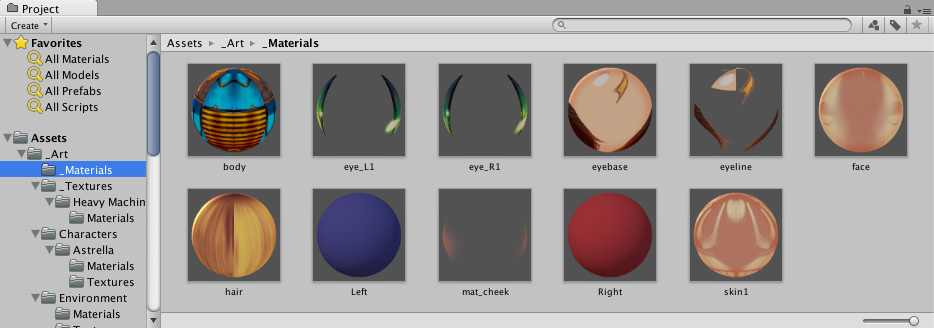
\includegraphics[width=0.6\linewidth,clip=]{slike/ProjectBrowser.jpg}
\figcaption{Prozor projekta}%
\label{fig:ProjectBrowser}%
\end{minipage}
\\[\intextsep]

S lijeve strane nalaze se direktoriji projekta prikazani u hijerarhijskoj listi. Klikom na neki od direktorija prikazuje se sadržaj tog direktorija na desnoj strani. Pojedini elementi su prikazani odgovarajućim ikonama tako da jednostavno možete pronaći potrebnu datoteku. Strukturu ovog prozora je lako prilagoditi vlastitim željama, moguće je povećati i smanjiti ikone, promijeniti vrstu prikaza, spremiti određene datoteke u favorite. Sve datoteke se mogu pretraživati unosom filtera, odnosno imena datoteku. Osim standardnog prikaza datoteka koje odgovaraju filteru pretraživanja, moguće je dodatno filtrirati rezultate pretraživanjem po tipu ili labelama. Klikom na datoteku prikazuju se detalji u nadglednom prozoru.

U prozoru scene nalazi se set navigacijskih kontrola koje olakšavaju rad unutar scene. U gornjem desnom kutu nalazi se naprava (engl.~\textit{Gizmo}).~\ref{fig:SceneGizmo}
\\[\intextsep]
\begin{minipage}{\linewidth}
\centering%
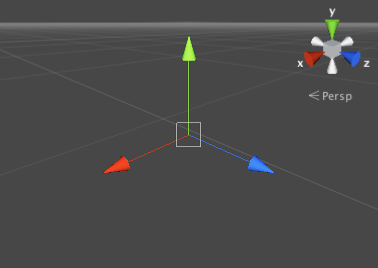
\includegraphics[width=0.6\linewidth,clip=]{slike/SceneGizmo.png}
\figcaption{Naprava (engl.~\textit{Gizmo})}%
\label{fig:SceneGizmo}%
\end{minipage}
\\[\intextsep]

S njim se mijenja perspektiva, odnosno pogled unutar scene, te na taj način možemo koristiti odgovarajuće postavke ovisno o tome što se trenutno radi u sceni.
Vrste pogleda su:
\begin{itemize}
 \item Perspektivni model,
 \item ortogonalni model,
 \item prednji pogled,
 \item topografski pogled.
\end{itemize}

Alat za rad s objektima~\ref{fig:UI-ViewTool}nalazi se u gornjem desnom kutu. Prva ikona predstavlja alat s kojim se kreće po sceni, takozvani (engl.~\textit{Hand tool}). A tu su i ostali botuni s kojima možemo rotirati, pomicati, te povećavati, odnosno smanjivati objekte.
\\[\intextsep]
\begin{minipage}{\linewidth}
\centering%

\includegraphics[width=0.6\linewidth,clip=]{slike/UI-ViewTool.png}
\figcaption{(engl.~\textit{UI-ViewTool})}%
\label{fig:UI-ViewTool}%
\end{minipage}
\\[\intextsep]

Neki od prečaca koji mogu ubrzati rad unutar scene nalaze se na slici~\ref{fig:SceneShortcuts}.
\\[\intextsep]
\begin{minipage}{\linewidth}
\centering%
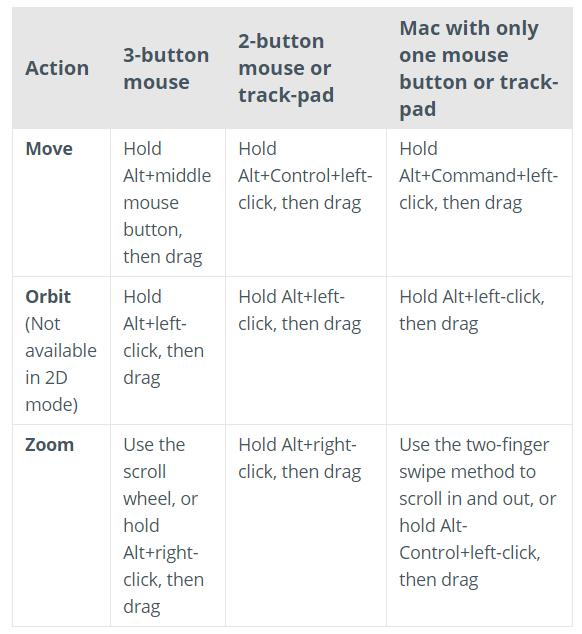
\includegraphics[width=0.6\linewidth,clip=]{slike/SceneShortcuts.png}
\figcaption{Prečaci za rad u sceni}%
\label{fig:SceneShortcuts}%
\end{minipage}
\\[\intextsep]

Jedna od jako korisnih stvari je (engl.~\textit{Unit snapping}) koji se koristi na način da se pritisne na kontrolnu tipku (engl.~\textit{Control-CTRL}) te onda koristeći alat za pomicanje ili transformiranje (kombinacija pomicanja, rotiranja i mijenjanja veličine) promijenimo vrijednost za onu koja je postavljena u postavkama (engl.~\textit{Snap settings}). 

Tijekom rada korisnik može uključiti, odnosno isključiti određene efekte unutar scene, ti efekti su prisutni jedino tijekom rada na projektu, te nemaju nikakvi utjecaj na završni proizvod, to su:
\begin{itemize}
 \item Crtače metode
	\begin{itemize}
	  \item (engl.~\textit{Shaded}) Prikazuje površine s teksturama,
	  \item (engl.~\textit{Wireframe}) prikazuje strukture objekata u obliku linija različitih boja,
	  \item (engl.~\textit{Shaded Wireframe}) kombinacija prethodna dva navedena.
	\end{itemize}
 \item Razno
	\begin{itemize}
	  \item Vidljivost sijena,
	  \item prikaz načina učitavanja tekstura.
	  \item prikaz transparentnih objekata.
	  \item prikaz idealne veličine tekstura ovisno o objektu (engl.~\textit{Mipmaps}).
	\end{itemize}
 \item Prikaz vrsta materijala,
 \item globalno osvjetljenje.
\end{itemize}

Postoji još nekoliko različitih mogućnosti što se tiče postavki tijekom rada, mijenjanje aktivnog osvijetljena, uključivanje, isključivanje ikoni kao i mijenjanje veličina ovisno o tome što vam je trenutno potrebno za rad na projektu. Na slici je prikazan izgled scene s aktivnim sličicama te rešetkama. ~\ref{fig:GizmoIGrid}.
\\[\intextsep]
\begin{minipage}{\linewidth}
\centering%
\includegraphics[width=0.6\linewidth,clip=]{slike/GizmoIGrid.png}
\figcaption{Rešetke i sličice (engl.~\textit{Grid and gizmo icons activated})}%
\label{fig:GizmoIGrid}%
\end{minipage}
\\[\intextsep]

Prozor igre je ono gdje se vidi konačni proizvod, prozor koji predstavlja konačno stanje igre. Da bi se moglo prikazati što se događa u igri potrebne su jedna ili više kamera, koje trebaju biti kontrolirane na način da korisnik može vidjeti, odnosno igrati igru. Kontrolni botuni igre omogućavaju pokretanje, pauziranje te zaustavljanje igre. Na slici ~\ref{fig:GameViewControlBar} prikazane su mogućnosti, odnosno postavke unutar prozora igre.
\\[\intextsep]
\begin{minipage}{\linewidth}
\centering%
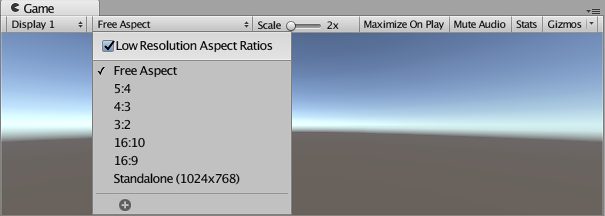
\includegraphics[width=0.6\linewidth,clip=]{slike/GameViewControlBar.png}
\figcaption{Mogućnosti prozora igre}%
\label{fig:GameViewControlBar}%
\end{minipage}
\\[\intextsep]

U tablici ~\ref{fig:OpcijeGameView} opisane su pojedine postavke. 
\begin{table}
\begin{tabularx}{0.9\textwidth}{lX}
\hline
Botun&Opis \\
\hline
Prikaz&Odabir kamere ukoliko 
imate više kamera unutar igre. \\
Odnos(engl.~\textit{Aspect})&Pregled izgleda na
 različitim veličinama ekrana.\\
Odabir niske rezolucije&Odaberite ovo ako želite vidjeti
 kako bi igra izgledala na starijim ekranima.\\
Povećalo&Mogućnost uvećanja,
 odnosno smanjenja prikaza. \\
Maksimiziranje ekrana&Ukoliko je ovo odabrano slika se 
automatski maksimizira tijekom pokretanja igre. \\
Zvuk&Gašenje zvuka po potrebi. \\
Statistika&Prikazuju se podaci o kvaliteti performansa tijekom igranja, 
podaci o grafici, memoriji, procesoru, jačini zvuka i slično.\\
\hline
\end{tabularx}
\caption{Opcije unutar prozora igre.}\label{fig:OpcijeGameView}
\end{table}

Početni izgled prozora hijerarhije nalazi se na slici ~\ref{fig:Hierarchy}. Prilikom stvaranja novog projekta tu se nalazi naziv scene, glavna kamera te glavni izvor osvijetljena u sceni.
\\[\intextsep]
\begin{minipage}{\linewidth}
\centering%
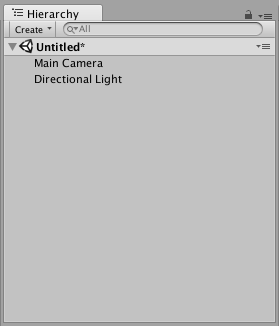
\includegraphics[width=0.6\linewidth,clip=]{slike/Hierarchy.png}
\figcaption{Početni izgled hijerarhijskog prozora}%
\label{fig:Hierarchy}%
\end{minipage}
\\[\intextsep]
Ovaj prozor sadrži listu svih objekata koji se nalaze unutar trenutne scene, tzv. (engl.\textit{GameObject}). Neki su obični 3D modeli dok su neki, tzv. (engl.\textit{Prefabs}), odnosno objekti koji se mogu spremiti te tako ponovo koristiti unutar scene, ili neke druge scene. Kada se objekti uklone ili dodaju iz scene tako se brišu, odnosno dodaju unutar hijerarhijskog prikaza. Po potrebi korisnik može mijenjati raspored objekata te isto tako mijenjati odnos dijete ili roditelj. Na slici ~\ref{fig:HierarchyParenting1} prikazan taj odnos, objekt koji je prvi u hijerarhiji, odnosno koji sadrži neke druge objekte je roditelj,a objekti koji su sadržani unutar roditelja su djeca.
\\[\intextsep]
\begin{minipage}{\linewidth}
\centering%
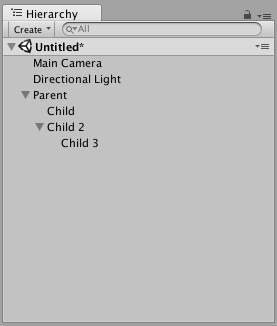
\includegraphics[width=0.6\linewidth,clip=]{slike/HierarchyParenting1.png}
\figcaption{Prikaz odnosna objekata}%
\label{fig:HierarchyParenting1}%
\end{minipage}
\\[\intextsep]

Da bi mijenjali odnos objekata jednostavno se povuče objekt na budući objekt roditelj. Više objekata na istoj razini su braća i sestre. Primjer je prikazan na slici ~\ref{fig:HierarchyParenting3}, objekt 1 je roditelj, objekti 2 i 3 su djeca. Njihov raspored se isto tako može mijenjati.
\\[\intextsep]
\begin{minipage}{\linewidth}
\centering%
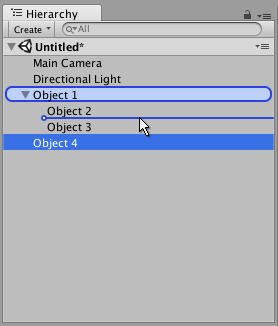
\includegraphics[width=0.6\linewidth,clip=]{slike/HierarchyParenting3.png}
\figcaption{Prikaz djece}%
\label{fig:HierarchyParenting3}%
\end{minipage}
\\[\intextsep]

Raspored objekata se može promijeniti tako da budu abecedno poredani, sve što je potrebno je promijeniti postavke izgleda hijerarhije. Isto tako je omogućeno uređivanje, odnosno prikaz više od jedne scene unutar iste hijerarhije.

Nadgledni prozor prikazuje detaljne informacije trenutno odabranog objekta, uključujući sve komponente koje su dodane na taj objekt, njihova svojstva te omogućava promjenu njihove funkcionalnosti u sceni. Na slici ~\ref{fig:GenericInspector} prikazan je nadgledni prozor s primjerom postavki te komponenti nekog objekta.
\\[\intextsep]
\begin{minipage}{\linewidth}
\centering%
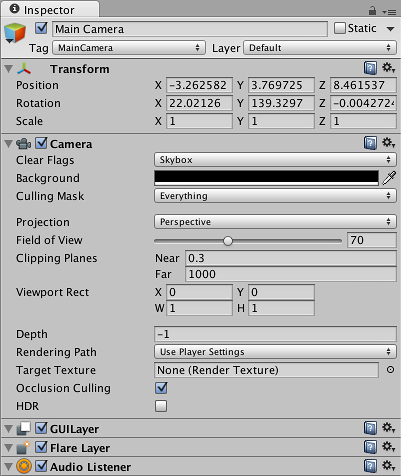
\includegraphics[width=0.6\linewidth,clip=]{slike/GenericInspector.png}
\figcaption{Nadgledni prozor}%
\label{fig:GenericInspector}%
\end{minipage}
\\[\intextsep]

Ovaj prozor se koristi za promjenu svojstava gotovo svega unutar Unityja, od objekata, materijala pa sve do postavki samog editora. Kada odaberete neki objekt unutar hijerarhije ili scene, nadgledni prozor prikazuje sva svojstva koja opisuju taj objekt, na slici~\ref{fig:PlayerInspector} prikazan je izgled prozora kada je odabran objekt igrač (engl.~\textit{Player}) osim podataka o položaju i veličini tu su prikazane i sve ostale komponente vezane za taj objekt, podaci o tome je li u pitanju fizički objekt, sadrži li neke od standardnih komponenti unutar Unityja kao što je sudarač (engl.~\textit{Collider}) i slično te naravno skripte koje pripadaju tom objektu, npr. "Player" skripta koja je prikazana na slici. Osim imena skripte tu su prikazane sve varijable koje su javne (engl.~\textit{Public}), nazivi te vrijednosti.
\\[\intextsep]
\begin{minipage}{\linewidth}
\centering%
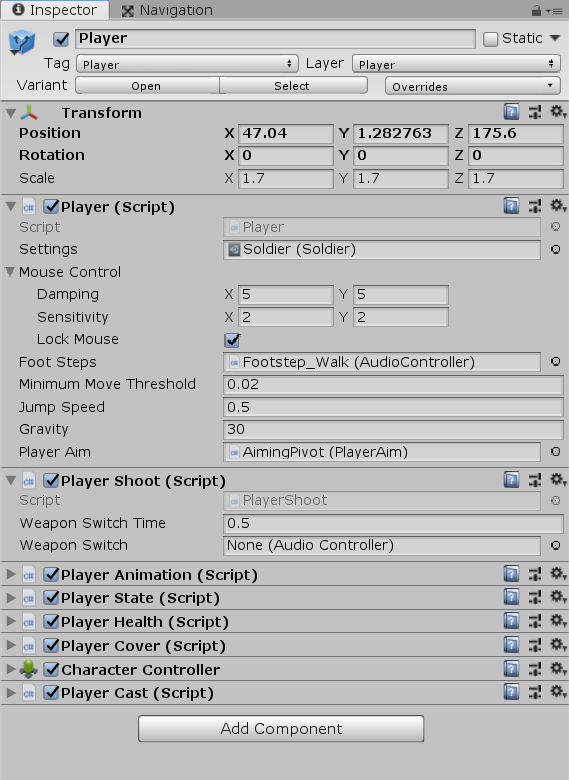
\includegraphics[width=0.6\linewidth,clip=]{slike/PlayerInspector.png}
\figcaption{Nadgledni prozor igrač (engl.~\textit{Player})}%
\label{fig:PlayerInspector}%
\end{minipage}
\\[\intextsep]

Na slici ~\ref{fig:InspectorExampleMaterial} prikazane su postavke za svojstvo objekta materijal. Najvažnije su postavke načina prikazivanja u sceni te dodavanja glavnih tekstura za objekt (engl.~\textit{Maps}).
\\[\intextsep]
\begin{minipage}{\linewidth}
\centering%
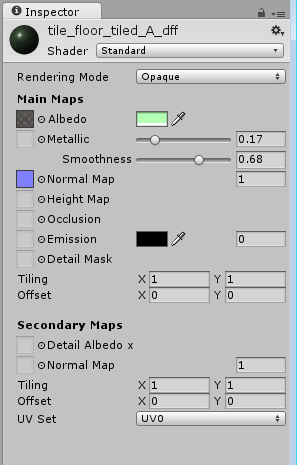
\includegraphics[width=0.6\linewidth,clip=]{slike/InspectorExampleMaterial.png}
\figcaption{Prikaz postavki za materijal}%
\label{fig:InspectorExampleMaterial}%
\end{minipage}
\\[\intextsep]

Komponente se na objekt dodaju vrlo jednostavno, samo treba pritisnuti botun dodaj komponentu (engl.~\textit{Add components}) te izabrati ono što je potrebno, a kada je riječ o dodavanju skripti tada je vrlo jednostavno možete povući iz projektnog prozora na sami objekt. Vrlo je važno paziti na ovisnosti o ako postoje, zbog toga što skripte koje ovise o nekim drugim dodaju automatski te skripte na objekt, a isto tako te skripte koje su dodane ne mogu se izbrisati jer postoji ovisnost s glavnom skriptom.

Kako bi se lakše snalazili u sceni, moguće je objektu pridružiti boju, odnosno sličicu koja se prikazuje iznad objekta, tako moguće je lakše vidjeti gdje se nalaze svi objekti tog tipa u sceni. Isto tako bilo koja slika koja je uključena u projekt može predstavljati sličicu. Primjer postavljene ljubičaste sličice za komponente kamera koje su vezane za vozilo, prikazan je na slici~\ref{fig:IconShow}.
\\[\intextsep]
\begin{minipage}{\linewidth}
\centering%
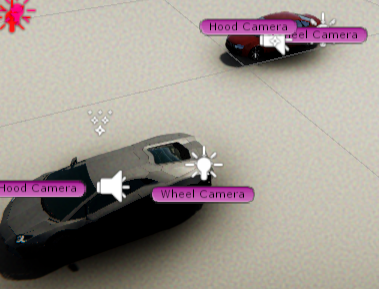
\includegraphics[width=0.6\linewidth,clip=]{slike/IconShow.png}
\figcaption{Primjer prikaza sličica s nazivom za objekte istog tipa}%
\label{fig:IconShow}%
\end{minipage}
\\[\intextsep]

Svaki objekt ima svoja svojstva, te se vrijednosti mogu mijenjati ovisno o potrebi. Kada se o objektima koji se koriste u svrhu uređenja scene, to su najčešće veličina, položaj, ima li objekt sudarač, njegov materijal i slično, dakle objekti koji su uglavnom statični. Isto tako ako se radi o objektima čija je svrha poboljšanje ugođaja igre, onda ti objekti najčešće imaju komponentu svjetlost, gdje možemo podesiti intenzitet, boju, radijus osvjetljenja i slično ili zvuka koji se može aktivirati prilikom nekog događaja, ili biti aktiviran konstantno tijekom igre. Druga vrsta objekata su objekti koji s kojima je omogućena interakcija, dakle objekti koji uglavnom sadrže neku skriptu preko koje im je definirana uloga unutar scene, odnosno igre, to mogu biti stvari, likovi, i slično. Prilikom igranja, aktiviraju se funkcionalnosti skripti koje su dodane na te objekte, to može biti kretanje, govor, uporaba alata itd.

Još jedna opcija nadglednog prozora je izbor normalnog načina rada ili rada za pronalaženje grešaka (engl.~\textit{Debug mode}). Način rada za pronalaženje grešaka se koristi kao i u svim programskim jezicima, služi za praćenje promjena stanja varijabli, možemo vidjeti i privatne varijable, ali ih ne možemo mijenjati.

Neki drugi prozori koji će naknadno biti opisani su:
\begin{itemize}
  \item Konzolni prozor,
  \item prozor animacija,
  \item prozor za praćenje performansi,
  \item prozor za osvjetljenje,
  \item Prozor za upravljanje s postavkama optimizacije (engl.~\textit{Occlusion Culling}).
\end{itemize}

\subsection{Stvaranje igre}
Ono što je jedna od posebnosti Unityja je što nije potrebno imati godine iskustva u kodiranju da bi napravili igricu. Uz praćenje i razumijevanje jednostavnih procesa izrade igre, u vrlom kratkom roku započet će te s izradom igara. 
U ovom poglavlju će biti opisan općeniti pristup radu na igri, bit će izdvojene glavne komponente, koje se najčešće koriste tijekom rada unutar Unityja, odnosno tijekom stvaranja igre. Većina ovih koncepata su bazirana na izradi skripti, što će kasnije biti detaljnije obrađeno.

Tijekom izrade igre, sva okolina i izbornici su sadržani unutar scena. Može se reći da je svaka scena jedinstvena razina (engl.~\textit{Unique level}). Unity sprema scene unutar direktorija sa svim dodacima, odnosno unutar prozora projekta gdje se nalaze svi ostali dodaci. Tijekom izrade igre važno je paziti na urednost projekta, tako da je korisno napraviti direktorij koji će sadržavati sve scene vezane za taj projekt.

Već je mnogo puta spomenut izraz objekt igrice (engl.~\textit{Game object}), to je naravno, s razlogom. Objekti su najvažniji dio Unityja, od likova, stvari pa do efekata, kamera i slično, međutim objekt sam po sebi ne može ništa raditi ako nema dodanu komponentu skripte u kojoj je programirana logika za taj objekt. Na slici~\ref{fig:GameObjectsExamples} prikazana su četiri različita tipa objekata. Objektima se trebaju pridružiti odgovarajuće komponente kako bi se postigla funkcionalnost koju je korisnik zamislio.
\\[\intextsep]
\begin{minipage}{\linewidth}
\centering%
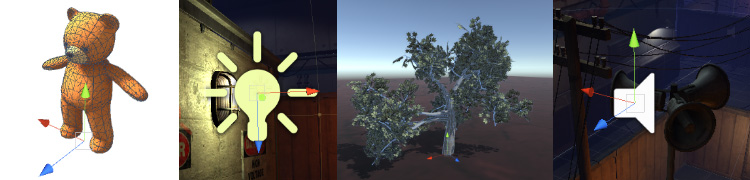
\includegraphics[width=0.6\linewidth,clip=]{slike/GameObjectsExamples.jpg}
\figcaption{animirani lik, svjetlost, stablo, izvor zvuka}%
\label{fig:GameObjectsExamples}%
\end{minipage}
\\[\intextsep]

Neke od najčešćih komponenti koje se koriste tijekom izrade igre su:
\begin{itemize}
  \item Podaci o položaju i veličini (engl.~\textit{Transform}) ,
  \item kruto tijelo (engl.~\textit{Rigidbody}),
  \item svjetlost,
  \item zvuk,
  \item kontroler lika,
  \item sudarač,
  \item učitavač oblika (engl.~\textit{Mesh renderer},
  \item kontroler animacije,
  \item C\# skripte.
\end{itemize}

Svi objekti se mogu aktivirati ili deaktivirati unutar scene preko nadglednog prozora, ali i unutar samih skripti, što je vrlo korisno, bilo da je u pitanju neki efekt koji je pridružen objektu te se treba aktivirati samo u određenom trenutku, bilo da je riječ o objektu koji se može uništiti, ali će se nakon nekog vremena ponovo pojaviti u igri.
Objektu se može pridružiti i tag, to je referentni naziv za određene objekte, npr. ako je potrebno, moguće je napraviti tag "Igrač" za sve likove kontrolirane od strane igrača te npr. tag "Neprijatelj", ako se radi o protivniku. To je vrlo korisno jer je tako moguće napisati logiku unutar koda, gdje će se različiti objekti ponašati na različiti način ovisno o tagu.

Na jednostavan način provjeravamo je li se objekt odgovarajućeg taga sudario s objektom kojeg je moguće skupiti, ako je, igrač će prikupiti stvar, a dalje je programski riješeno ponašanje ovisno o prikupljenoj stvari. Primjer k\^oda je dan u ispisu~\ref{primjerTag}. 

\begin{lstlisting}[caption={Uporaba taga}, label=primjerTag]
public class PickupItem : MonoBehaviour {

    void OnTriggerEnter(Collider collider)
    {
        if (collider.tag != "Player")
        {
            return;
        }
        Pickup(collider.transform);
    }

    public virtual void OnPickup(Transform item)
    {
        print("colliding");
    }

    void Pickup(Transform item)
    {
        OnPickup(item);
    }
}
\end{lstlisting}

Nove tagove je vrlo jednostavno dodati preko nadglednog prozora, gdje se preko padajućeg izbornika pristupa tagovima, te odabere opcija "dodaj tag". Svaki objekt može imati samo jedan tag. A i Unity ima određene tagove već napravljene, to su uobičajeni tagovi koji se koriste tijekom izrade igre:
\begin{itemize}
  \item Untagged,
  \item Respawn,
  \item Finish,
  \item EditorOnly,
  \item MainCamera,
  \item Player,
  \item GameController.
\end{itemize}

Jedno od vrlo važnih svojstava objekata je, jesu li statični ili ne, to svojstvo je bitno kad je u pitanju optimizacija. A govori nam može li se objekt micati ili ne. Tako neka svojstva, kad je riječ o performansama mogu biti unaprijed izračunata, odnosno optimizirana. To se u pozadini izvršava tako da se više statičnih objekata poveže u jedan veliki objekt zvan gomila (engl.~\textit{Batch}). Na slici ~\ref{fig:GameObjectStaticDropDownMenu} je prikazan nadgledni prozor s padajućim izbornikom gdje imamo različite opcije kada su u pitanju postavke statičnih objekata.
\\[\intextsep]
\begin{minipage}{\linewidth}
\centering%
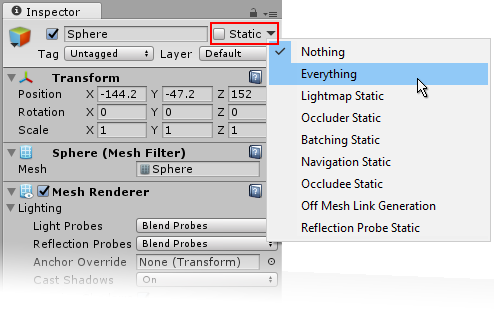
\includegraphics[width=0.6\linewidth,clip=]{slike/GameObjectStaticDropDownMenu.png}
\figcaption{Izbornik za odabiranje različitih svojstva statičnih objekata}%
\label{fig:GameObjectStaticDropDownMenu}%
\end{minipage}
\\[\intextsep]

Tijekom rada na projektu, u nekom trenutku će biti potrebno napraviti izvršnu datoteku za testiranje dosadašnjeg rada, u tom slučaju je potrebno pristupiti postavkama za izradu projekta, dakle za stvaranje izvršne datoteke. Potrebno je dodati sve scene koje korisnik želi uključiti u datoteku, te ih poredati redoslijedom kakvim želite da se učitavaju. Svaka scena ima, osim naziva i indeks, koji se inkrementira kako se dodaju scene. To je bitno kada u programskom rješenju želite pristupiti određenoj sceni u trenutku izvršavanja određene radnje.
Ako želite napraviti projekt koji se može pokretati na različitim plaformama treba uzeti u obzir da igra napravljena za računalo, koja ima stabilne performanse ne mora se jednako ponašati na mobilnim uređajima, iz jednostavnog razloga što mobiteli nemaju jednaku procesorsku moć kao računala.
Na slici ~\ref{fig:SavingBuildSettings} prikazan je izgled prozora prilikom stvaranja izvršne datoteke, važno je napomenuti da treba izabrati odgovarajuću platformu za koju želite napraviti datoteku.
\\[\intextsep]
\begin{minipage}{\linewidth}
\centering%
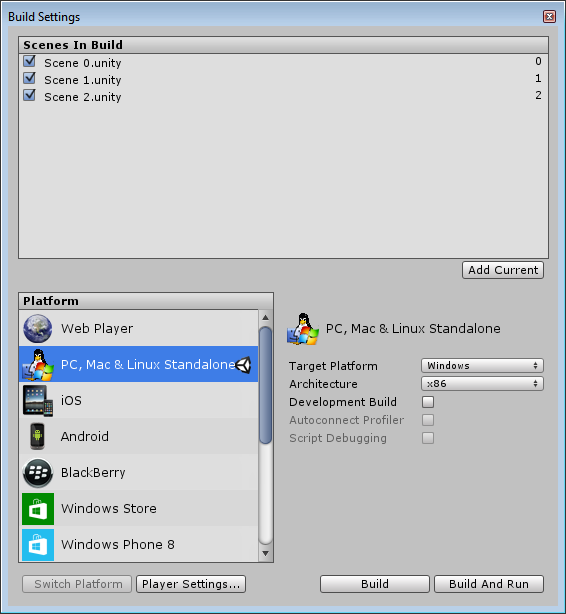
\includegraphics[width=0.6\linewidth,clip=]{slike/SavingBuildSettings.png}
\figcaption{Prozor s postavkama za izradu izvršne datoteke}%
\label{fig:SavingBuildSettings}%
\end{minipage}
\\[\intextsep]

Unity ima sistem koji omogućava stvaranje već gotovih uzoraka koji se kasnije mogu jednostavno upotrebljavati kada su god potrebni, sa svom djecom, komponentama te svojstvima koji opisuju taj objekt. To su tzv. uzorci (engl.~\textit{Prefabs}).
Kada želite ponovno koristiti neki objekt konfiguriran na određeni način, npr. lik kojeg ne kontrolirate (engl.~\textit{NPC-non-player character}), ili možda određeni objekt koji je dio garniture, ali ga želite koristiti i u nekim drugim scenama onda je preporučljivo taj objekt pretvoriti u uzorak, tako ste sigurni da je taj objekt jednak u svim svojim pojavljivanjima. To je puno bolje od standardnog kopiranja nekog objekta, jer svaka promjena na uzorku se propagira na sve uzorke gdje god da se pojavljuju. Isto tako je moguće određenu instanciju prilagoditi ovisno o potrebi scene te napraviti varijantu tog uzorka.
Uz već navedene primjere korištenja uzoraka, uobičajeni primjeri su još instanciranje projektila, ili glavnog lika u igri, npr. uzorak igrača može se nalaziti na polaznoj točki svake scene. Na slici ~\ref{fig:PlayerPrefab} prikazan je uzorak Igrača.
\\[\intextsep]
\begin{minipage}{\linewidth}
\centering%
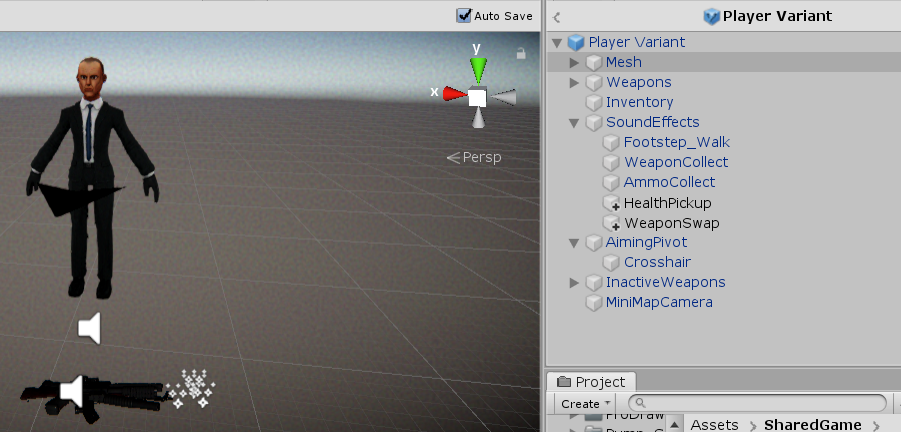
\includegraphics[width=0.6\linewidth,clip=]{slike/PlayerPrefab.png}
\figcaption{Uzorak Igrača}%
\label{fig:PlayerPrefab}%
\end{minipage}
\\[\intextsep]

Stvaranje uzorka je vrlo jednostavan proces, željeni objekt se povuče iz prozora hijerarhije u prozor projekta i stvoren je uzorak tog objekta. Ako postoji već uzorak tog objekta, onda možete odabrati hoće li to biti varijanta uzorka, ili novi uzorak. Sada kada god poželite možete povući taj uzorak ili direktno u scenu ili u hijerarhiju te će se instancirati taj objekt. Objekti koji su uzorci, prikazani su plave boje.
Ako želite urediti uzorak, jednostavno duplim klikom na objekt ulazite u prozor za uređivanje uzorka, u trenutku kada ste gotovi, odnosno izađete iz prozora za uređivanje, promjene se automatski spremaju, tu opciju možete isključiti te spremati ručno.
Kao što je već spomenuto instance uzoraka se mogu prilagoditi ovisno o potrebi, a onda ako želite moguće je potvrditi promjenu na uzorku, ili vratiti na početnu vrijednost uzorka, to je moguće i desnim klikom na pojedine komponente.
Ako je neki objekt uzorak, a ne želite da bude više onda je potrebno raspakirati taj objekt. Desnim klikom na objekt pritisnite raspakiraj i objekt više neće biti uzorak, to ne znači da je izbrisan taj uzorak, već ta instanca više nije uzorak, nego slobodni objekt.

Prethodno je objašnjeno kako koristiti mogućnosti uzoraka na razini editora, u nastavku će biti opisani neki primjeri kada je korisno koristiti uzorke i unutar skripti. Jedan od primjera je izgradnja zida, skripta ~\ref{IzgradiZid} prikazuje kako bi pristupili izradi zida, bez korištenja uzorka.

\begin{lstlisting}[caption={Skripta za izradu zida}, label=IzgradiZid]
public class Instantiation : MonoBehaviour 
{
    void Start()
    {
        for (int y = 0; y < 5; y++) 
        {
            for (int x = 0; x < 5; x++) 
            {
                GameObject cube = GameObject.CreatePrimitive(PrimitiveType.Cube);
                cube.AddComponent();
                cube.transform.position = new Vector3(x, y, 0);
            }
        }
    }
}
\end{lstlisting}

Skripta se doda na prazan objekt te nakon što se pokrene igra, izgradi se zid. Problem je u tome što ovakvim pristupom, svaka promjena na zidu, bilo to dodavanje tekstura, mijenjanje fizičkih svojstava, trenja i slično je nova linija k\^oda.
Koristeći uzorke prvo uredimo objekt na način koji želimo te se onda u skripti oslanjamo na taj uzorak, primjer skripte~\ref{NoviZid}.

\begin{lstlisting}[caption={Skripta za izradu zida koristeći uzorke}, label=NoviZid]
//Instantiate accepts any component type, because it instantiates the GameObject 
//brick is reference to prefab model

public Transform brick;

void Start() 
{
    for (int y = 0; y < 5; y++)
    {
        for (int x = 0; x < 5; x++) 
        {
            Instantiate(brick, new Vector3(x, y, 0), Quaternion.identity);
        }
    }
}
\end{lstlisting}

Ovim pristupom, ne samo da je skripta urednija, već sve promjene koje želimo napraviti na uzorku, ne radimo preko koda već direktno na tom uzorku, te prilikom novog pokretanja igre, zid nastaje sa svim novim svojstvima.

Drugi primjer je instanciranje projektila, projektil može imati različita svojstva, kao što su trag koji ostavlja iza sebe, zvuk, trag koji nastaje nakon sudara, svjetlost i slično, sve se to može i programski riješiti, međutim puno jednostavnije je napraviti uzorak sa svim potrebnim efektima, a unutar skripte samo instancirati taj objekt kada je potrebno npr. skripta~\ref{Metak}

\begin{lstlisting}[caption={Instanciranje metka}, label=Metak]
void CheckDestructable(RaycastHit hitInfo)
    {
        var destructable = hitInfo.transform.GetComponent();

        destination = hitInfo.point + hitInfo.normal * .01f;

        if (hitInfo.transform.tag == "Enemy" || hitInfo.transform.tag == "Player")
        {
            Transform blood = Instantiate(bloodImpact, destination, Quaternion.LookRotation(hitInfo.normal) * Quaternion.Euler(0,180f,0));
           
            flag = true;
        }
        else if (flag == false)
        {
            Transform hole = Instantiate(bulletHole, destination, Quaternion.LookRotation(hitInfo.normal) * Quaternion.Euler(0, 180f, 0));
            hole.SetParent(hitInfo.transform);
        }

        if (destructable == null)
        {
            return;
        }
        destructable.TakeDamage(damage);
        flag = false;
    }
\end{lstlisting}

Treći primjer je korištenje lutki (engl.~\textit{Ragdoll}), odnosno smrt neprijatelja i slično. Dakle igrač ubije neprijatelja, koji sadrži razne skripte i komponente koje su potrebne za funkcioniranje, i u slučaju smrti trebamo smisliti logiku što s tim likom. Jedna od opcija je deaktiviranje s komponenti i slično, međutim puno bolji pristup je brisanje tog objekta te instanciranje uzorka koji će npr. pokrenuti animaciju smrti, te će predstavljati mrtvo tijelo. Slična logika se može primijeniti kada su u pitanju vozila itd. Ovim pristupom puno je manja vjerojatnost neočekivanog ponašanja objekata u igri, čišći je k\^od i najvažnije jednostavno ga je ponovno upotrijebiti.

Unity podržava sve standardne uređaje za unos, dakle kada je riječ o kontrolama igre, unos može biti preko tipkovnice, kontrolera, miša te svi standardni načini unosa ako je riječ o mobilnim igrama.
Osim standardnih postavki za kontrole, moguće je definirati vlastite za kontrole, sve što je potrebno je promijeniti vrijednost u postavkama na slici~\ref{fig:InputAxis} te se referirati na taj botun preko skripte.
\\[\intextsep]
\begin{minipage}{\linewidth}
\centering%
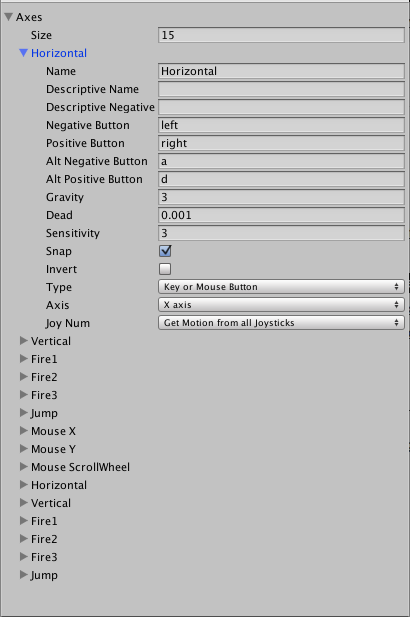
\includegraphics[width=0.6\linewidth,clip=]{slike/InputAxis.png}
\figcaption{Postavke kontrola}%
\label{fig:InputAxis}%
\end{minipage}
\\[\intextsep]

Rotacija i orijentacija su u 3D aplikacijama prikazna na jedan od dva načina, Kvaternionski ili Eulerovi kutovi. Svaki ima svoje koristi, ali i nedostatke. Unity koristi Kvaternione iznutra zbog toga što njihove prednosti nadvladavaju mane, ali prikazuje ekvivalentne vrijednosti Eulerovih kutova u nadglednom prozoru, tako da ih je jednostavno uređivati.
Razlika je u tome što je Eulerove lakše predstaviti, a to su tri kutne vrijednosti za X, Y i Z koje se uzastopno dodjeljuju. Da bi primijenili Eulerovu rotaciju objektu, svaka vrijednost se dodjeljuje redom, kao rotacija oko odgovarajuće osi.

Prednosti su što je čovjeku intuitivnije protumačiti ovaj format, te je moguće prikazati rotaciju veću od 180 stupnjeva. Limitacija je ta što kada se dodjeljuju tri rotacije po krugu, moguće je da prva ili druga rotacija po trećoj osi usmjeravaju u istom smjeru kao neka od prethodnih osi, izgubljen je tzv. stupanj slobode jer se treća vrijednost rotacije ne može dodijeliti jedinstvenoj osi. To je gimbalno zaključavanje (engl.~\textit{Gimbal lock}).

Kvaternioni se mogu koristiti kako bi se prikazala orijentacija ili rotacija objekta. Ovaj prikaz u pozadini sadrži četiri broja, u Unityju su to x, y, z i w. Ovi brojevi ne predstavljaju kuteve ili osi, i uglavnom im nikad ne trebamo pristupati direktno. Isto kao što vektor može prikazivati poziciju ili smjer (gdje je smjer izmjeren od izvora), Kvaternion može prikazivati orijentaciju ili rotaciju, a baš zbog toga što se vrijednosti mjere od rotacijskog izvora Kvaternion ne može prikazivati rotaciju iznad 180 stupnjeva.

Prednost je što Kvaternion ne može uči u gimbalno zaključavanje, a limitacije već spomenuto ograničenje rotacije, a osim toga brojevni prikaz Kvaterniona nije intuitivan.
Prilikom obrađivanja rotacije u skriptama, preporučljivo je koristiti Kvaternion klasu (engl.~\textit{Quaternion}). Unutar klase nalazi se mnoštvo korisnih metoda kao što su:
\begin{itemize}
  \item Quaternion.LookRotation,
  \item Quaternion.AngleAxis,
  \item Quaternion.FromToRotation,
  \item Quaternion.Slerp,
  \item Transform.Rotate,
  \item Transform.RotateAround.
\end{itemize}

\subsection{Grafika i optimizacija}
Unity ima set različitih postavki kvalitete grafike u namjeri da se poboljša učitavanje i performanse. Općenito govoreći, visoka kvaliteta znači i lošije performanse na starim slabim računalima i mobilnim uređajima, zato nije uvijek pametno ciljati na najbolji izgled igre. U postavkama za kvalitetu nalazi se matrica gdje su stupovi različite platforme,a reci razina kvalitete, što je prikazano na slici~\ref{fig:QualSettingsTop}. Moguće je dodati i vlastite postavke, kao i urediti ili izbrisati već postojeće.
\\[\intextsep]
\begin{minipage}{\linewidth}
\centering%
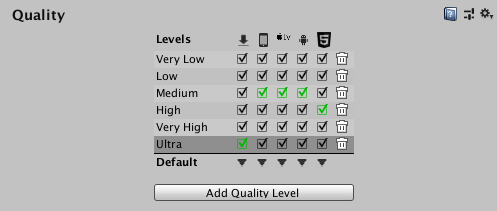
\includegraphics[width=0.6\linewidth,clip=]{slike/QualSettingsTop.png}
\figcaption{Prikaz postavki grafike}%
\label{fig:QualSettingsTop}%
\end{minipage}
\\[\intextsep]
Kada se dodaju vlastite postavke grafike, važno je podesiti učitavanje, dakle postavke kao što su, broj piksela svjetla, kvaliteta tekstura, uglađeni rubovi, refleksije i slično.
Postavke vezane za sjene, kao što su kvaliteta sjena, rezolucija, projekcija udaljenost itd.
Ostale postavke su vezane za broj kostiju lika koje sudjeluju u animaciji, osvježavanje, maksimalan broj zraka za aproksimiranje prašine, razine detalja i slično.

Grafika je vrlo bitan segment izrade igara, kako u pitanju izgleda igre, koji će ne samo lijepo izgledati, već biti pristupačan, odnosno zanimljiv igraču, tako je i važno voditi računa o limitacijama platformi za koje je igra napravljena. Samim time u pitanju je vrlo širok pojam, ovdje će biti opisani samo najvažniji pojmovi koji su bili korišteni u projektu kao što su modeli, svjetlost, efekti te na kraju malo o optimizaciji.

Generalno pričajući problem nastaje kada se pokušava postići vrhunska kvaliteta grafike, a zanemaruju se performans igre bude, tada bez obzira na lijepu igru, igrač ne može u potpunosti uživati u doživljaju.

Poželjno je da su modeli koji se koriste unutar projekta isto tako optimizirani, to se najviše odnosi na teksture, kvalitetno odrađeni modeli, najčešće imaju jednu veliku tzv. atlas mapu koja je napravljena od više različitih tekstura. To omogućava da se određeni dijelovi okoline mogu prikazati kao jedan veliki objekt, ali i dalje sa svim svojim detaljima. Loš pristup je mnogo tekstura koje su raspoređene pojedinačno na različitim objektima, dok je s tim postignut vrlo lijep izgled objekta, problem nastaje kada je u sceni mnogo takvih objekata. Svi objekti trebaju biti učitani, kako grafički tako procesorski predstavljeni u igri, a to izaziva loše performanse igre.

Svjetlost djeluje na način da osvjetljuje predmet, te taj predmet reflektira svjetlost, a u pozadini stvara sjenu. Baš kao u stvarnom svijetu, međutim nije baš jednostavno postići realnu scenu, treba voditi računa o više stvari, kao što je već spomenuto, platforme su limitirane, te je vrlo važno odabrati način na koji će se svjetlost obrađivati. Postoje dva ključna pojma po tom pitanju, a to su predizračunata i svjetlost u stvarnom vremenu. Tri su vrste izvora svjetlosti, to su direktna svjetlost, reflektor te snop. Ovisno o situaciji tijekom izrade vrlo je važno odabrati pravi izvor. Navedena tri spadaju u svjetlost u stvarnom vremenu, i koriste se za osvjetljavanje objekata. Problem je što ovim osnovnim principom ne možemo postići dovoljno visoku kvalitetu osvjetljenja, sjene su kompletno crne i pikseliziranih rubova, nema reflektiranog svjetla, i samo površine neposredno uz objekt su pod utjecajem, što je prikazano na slici~\ref{fig:RealtimeSpotlight}.
\\[\intextsep]
\begin{minipage}{\linewidth}
\centering%
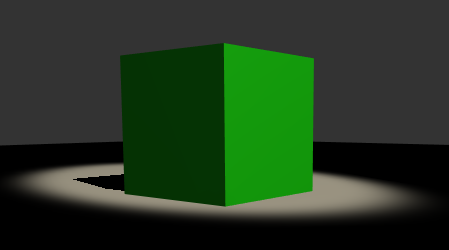
\includegraphics[width=0.6\linewidth,clip=]{slike/RealtimeSpotlight.png}
\figcaption{Osnovno osvjetljenje kocke}%
\label{fig:RealtimeSpotlight}%
\end{minipage}
\\[\intextsep]
Unity može izračunati kompleksne statičke svjetlosne efekte korištenjem tehnike globalne iluminacije te ih sprema u referentnu teksturnu mapu zvanu svjetlosna mapa (engl.~\textit{lightmap}) to je tzv. prženje svjetlosti (engl.~\textit{baking}. Prilikom ovog procesa, efekti svjetlosti koji nastaju djelovanjem na objekte u sceni koji su označeni kao statični izračunati su te upisani u teksturu koja je preko cijele scene te stvara geometriju svjetlosnih efekata, što je prikazano na slici ~\ref{fig:Lightmap}. Lijevo je prikazana jednostavna scena gdje je primijenjena svjetlosna mapa, a desno tekstura koja je generirana. Koristeći ovu metodu, efekti svjetlosti na odabrane objekte se ne mogu mijenjati.
\\[\intextsep]
\begin{minipage}{\linewidth}
\centering%
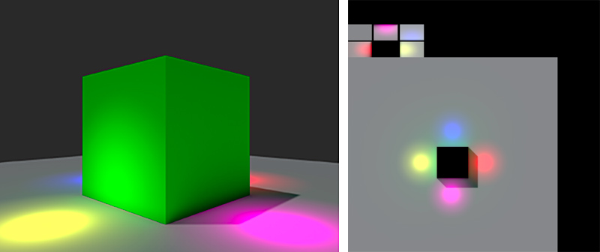
\includegraphics[width=0.6\linewidth,clip=]{slike/Lightmap.png}
\figcaption{Efekti svjetlosne mape}%
\label{fig:Lightmap}%
\end{minipage}
\\[\intextsep]

Ako želimo postići stvarno vremensku promjenu efekta svjetlosti, dakle dinamičko osvjetljenje trebamo koristiti predizračunatu stvarno vremensku globalnu iluminaciju. Dodatni alati koji pospješuju osvjetljenje su svjetlosne i reflektivne sonde. Svjetlosne sonde pojačavaju efekt svjetlosti, odnosno prikupljaju informacije o praznom prostoru gdje prolazi svjetlost. Reflektivne sonde prikupljaju informacije o refleksijama koje različite površine stvaraju, npr. u prostoriji gdje je mnoštvo metalnih površina, stakala i slično, korištenjem ove tehnike moguće je postići realnu scenu.

Sve ovo bilo bi beskorisno da na neki način ne možemo prikazati scenu, naravno za to su potrebne kamere. Svaka scena da bi se mogla prikazati treba imati najmanje jednu kameru, standardna svojstva kamere su pozicija, rotacija, kut prikaza, način na koji obrađuje svjetlost i slično. Kamera se može koristiti kao objekt koji osluškuje zvukove, a ono što je jako bitno svojstvo kamere je mogućnost da obrađivanja samo onog što je u kutu pregleda, dok se ostali dijelovi scene procesorski ne obrađuju, to svojstvo se naziva (engl.~\textit{Occlusion culling}). Kamera sama po sebi prikazuje scenu bez dodatnih efekata, međutim dodavanjem komponente za naknadno obrađivanje slike (engl.~\textit{Post-processing effect}) moguće je stvoriti mnoštvo zanimljivih efekata. Ovisno o stilu igre koji želite dobiti, mijenjanjem različitih postavki ove komponente moguće je zaista oživjeti scenu, kompletno dočarati željenu atmosferu u određenom dijelu vaše igre. Ono što će vam sigurno pomoći tijekom izrade igre je činjenica da što kamera ne vidi, nije vidljivo niti igraču, korištenjem ovog znanja, moguće je zamaskirati različite situacije unutar igre.

Vrijedno je navesti još jednu komponentu koja se može koristiti kako bi se dodatno uljepšalo scenu, to je sistem prašine. Osim onog što sami naziv sugerira, ova komponenta se može koristiti za predstavljanje bilo kakvog dinamičkog efekta, u samom projektu, korišten je za izradu efekta pucanja, prašine u skladištu, efekta eksplozije, krvi itd.

Naravno kao što je već spomenuto, performanse igre su vrlo bitne, a u želji da se postigne što bolje osvjetljenje i efekte treba paziti da to ne uzrokuje veliko pogoršanje. 
Unity ima ugrađen alat za praćenje performansa tijekom igranja, ali isto tako postoje vrlo dobri alati od treće strane, jedan od njih je Graphy, to je besplatni alat, korišten je tijekom izrade ovog projekta, i možete preuzeti sa stranica Unity trgovine s dodacima \url{https://assetstore.unity.com/packages/tools/gui/graphy-ultimate-fps-counter-stats-monitor-debugger-105778}, autor je Tayx.
Lista ispod navodi ključne točke kada su u pitanju performanse te s tim završava poglavlje vezano za grafiku.
\begin{itemize}
  \item Držati broj vrhova između 200 tisuča i 3 milijuna.
  \item Održavati što manju kompleksnost i manji broj materijala.
  \item Postaviti zastavicu za statičke objekte.
  \item Pržiti svjetlosne mape.
  \item Koristiti jedno direktno svjetlo.
  \item Koristiti kompresirane teksture te teksturne mape.
  \item Gdje god je moguće koristiti okluziju prikaza.
  \item Koristiti manje kompleksne modele i animacije gdje je moguće.
\end{itemize}

Osim o grafičkoj kvaliteti igre, važno je voditi računa i o veličini završnog projekta. Načelno, najviše memorije zauzimaju teksture, zvukovi i animacije, dok skripte manje utječu na veličinu projekta. 
Prvi korak prema manjoj veličini projekta je kompresija tekstura, osim toga moguće je smanjiti fizičku veličinu teksture, odnosno smanjiti broj piksela. U postavkama je potrebno smanjiti maksimalnu veličinu te pri tom paziti da objekt koji koristi texture bude prepoznatljiv.
Osim tekstura, moguće je komprimirati animacije, te tako dodatno uštedjeti na prostoru, treba uzeti u obzir da je to samo smanjenje veličine datoteke.

Kako bi spremili veliku količinu podataka, vrlo je dobra i korisna praksa koristiti skriptirane objekte (engl.~\textit{ScriptableObject}. To su podaci koji nisu vezani za instancu klase. Skriptirani objekti se najčešće koriste kada želite uštedjeti na memoriji, umjesto stvaranja dupliciranih vrijednosti i spremanja istih u standardne skripte, moguće je napraviti skriptirani objekt za spremanje tih vrijednosti, tako svi objekti preko reference pristupaju tim podacima. Osim toga, skriptirani objekti su korisni kada je potrebno spremiti određene podatke tijekom igranja. Skriptirani objekti se ne pridružuju objektima igre poput standardnih skripti, već se spremaju kao dodaci unutar projekta.
Primjer korištenja je prikazan u skripti ispod, skripta ~\ref{CreateScriptableObject} prikazuje kako se stvara skriptirani objekt, a kako bi koristili te objekte, sve što je potrebno je referencirati se na taj objekt unutar skripte gdje ćemo koristiti te podatke.

\begin{lstlisting}[caption={Stvaranje skriptiranog objekta}, label=CreateScriptableObject]
using UnityEngine;

[CreateAssetMenu(fileName ="Soldier",menuName ="Data/Soldier")]
public class Soldier : ScriptableObject {

    public float RunSpeed;
    public float WalkSpeed;
    public float CrouchSpeed;
    public float SneakSpeed;
}
\end{lstlisting}

Osim stvaranja skriptiranog objekta, na ovaj način smo dodali u Unity editor direktan pristup izradi nove datoteke koja će sadržavati potrebne postavke.
Isto tako je moguće stvoriti vlastite prozore, sve što je potrebno je napraviti skriptu koja nasljeđuje klasu EditorWindow, te implementirati grafičko sučelje. Iako ova mogućnost nije korištenja u projektu, jako je korisna, jer na ovaj naćin moguće je napraviit prozore koji se ponašaju slično kao npr. nadgledni prozor, gdje će se pregledavati i uređivati svojstva važna za projekt.

\subsection{Fizika, animacije, navigacija i skripte}
Kako bi se postigla realna fizika potrebno je postiči da objekt ubrzava ispravno, da na njega utječe kolizija, gravitacija i druge sile. Unity ima već ugrađene komponente koje se brinu baš o tim segmentima, samo s nekoliko postavki moguće je postiči realno ponašanje. Kontroliranjem fizike preko skripti, moguće je objektu dodjeliti dinamike vozila, stroja, pa čak i komada odječe.
Unity ima dva različita sistema obrađivanja fizike, 3D i 2D fizika, glavni koncepti su uglavnom isit, međutim implementirani su različitim komponentama, npr. kada je riječ o 3D postoji Rigidbody komponenta, a analogno tome Rigidbody 2D za 2D fiziku.

Čvrsto tijelo (engl.~\textit{Rigidbody}) (u nastavku će se koristiti engleski naziv), je glavna komponenta koja omogućava fiziku objekta. Dodjeljivanjem ove komponente objektu, automatski je pod utjecajem gravitacije, a ako se doda i sudarač (engl.~\textit{Collider}) onda je i pod utjecajem kolizije s ostalim objektima.
Iz skripte kontroliramo ove objekte dodavanjem sile koja gura objekt, što znači da nije poželjno mijenjati poziciju preko skripte, već će se ugrađeni alat za obrađivanje tih rezultata pobrinuti o novoj poziciji objekta. Naravno nekad ćemo htjeti sami pomaknuti objekt na određenu poziciju, ali kada je riječ o standardnim kretanjama koje želimo postići sa objektom, potrebno je samo navesti vrijednost sile koja će djelovati na taj objekt, te odrediti smjer.

Kao što postoje primitivni oblici tako postoje i primitivni sudarači, a to su kocka, kugla i kapsula, u večini slučajeva ovi sudarači su dovoljni, odnosno moguće ih je koristiti za večinu objekata u sceni. Dakle u slučaju da želimo omogućiti sudaranje s drugim objektima moramo dodati ovu komponentu. Nekada, ako je objekt previše kompleksan i želimo postići što realnije sudaranje, trebamo koristiti kompleksni sudarač koji se temelji na obliku samog objekta za kojeg želite koristiti ovaj sudarač (engl.~\textit{Mesh collider}). Ovi sudarači su naravno teži za obrađivanje te je gdje je god moguće poželjno koristiti primitivne sudarače.
Sudarači se koriste za tlo, zid, objekte kroz koje nije moguće proči i slično. Ovo su tzv. statički sudarači, dakle objekti koji se ne mogu pomicati u sceni. Ako se radi o objektu koji se može micati, odnosno ima komponentu Rigidbody, tada se radi o dinamičkim sudaračima. Efekt sudaranja ovisi o tome jesu li statički ili dinamički.
Kada se dogodi interakcija između sudarača, onda ovisno o površini i svojstvima iste, rezultat tog sudaranja je različit. Npr. ako se radi o površini kao što je led, onda će biti vrlo skliska, a ako je riječ o gumenoj površini, onda bi trebala pružiti dosta trenja itd. Postizanje ovih efekata nije baš jednostavno te zahtjeva dosta testiranja, ali moguće je postiči jako realne rezultate. 
Sudarači, osim uloge koju imaju vezano za fiziku, jako su korisni kada su u pitanju programska riješenja različitih situacija u igri. Svaki sudarač ima svojstvo okidanja (engl.~\textit{Trigger}) ovo svojstvo kada je postavljeno, tada sudaranjem s istim moguće je aktivirati različite događaje. Npr. ulaženjem u okidač moguće je aktivirati ispis nekog teksta na ekranu, ili pokretanje kratkog filma unutar igre i slično. Baš ovo svojstvo je korišteno u projektu na velik broj različitih načina te će to biti predstavljeno u dijelu gdje će biti opisana igra i korištena programska riješenja.
Lista navodi metode koje su dostupne kada su u pitanju okidači.
\begin{itemize}
  \item OnCollisionEnter,
  \item OnCollisionStay,
  \item OnCollisionExit,
  \item OnTriggerEnter,
  \item OnTriggerStay,
  \item OnTriggerExit.
\end{itemize}

Svaki lik kontroliran od strane igrača, kao i ostali koji se korise u igri trebaju neku vrstu fizike bazirane na sudaranju. Npr. mogućnost kretanja, onemogučavanje propadanja kroz tlo, ili prolaženje kroz zidove. Kada se radi o 3D fizici, ovo ponašanje može se stvoriti korištenjem komponente kontroler lika (engl.~\textit{Character Controller}). Ova komponenta daje liku jednostavni sudarač u obliku kapsule koji je uvijek usmjeren prema gore te sami kontroler ima vlastite specijalne funkcionalnosti kao što su brzina i smjer, objekt koji sadrži ovu komponentu ne može prolazit kroz statičke sudarače, može detektirati uzvišene površine, pomicati ostale objekte koji na sebi imaju Rigidbody komponentu, ali neče mu se mijenjati akceleracija ovisno o tome sudari li se s nekim objektom itd. Ova komponenta je korištena na glavnom liku igre.

Sistem animacija unutar Unityja je napredan sustav s potpunom kontrolom animacija tijekom igranja, pozivanje eventa pomoću animacija, sofisticirani sistem stanja (engl.~\textit{State machine}), tranzicija, povezivanja više stanja u jednu animaciju itd. Osim toga, cijeli sistem je vrlo jednostavan i intuitivan, uz mogućnost pregledavanja animacija i prijelaza unutar pomoćnog prozora, povezivanje animacija s jednostavnim dodavanjem prijelaza, te opisivanja istih koristeći pomoćne varijable, kao što su provjera je vrijednosti istina i laž, okidači te vrijednosti parametara kada je u pitanju pokretanje itd. Animacije se mogu uvoziti u Unity od softvera treće strane, kao i one napravljene u Unityju. Moguće je koristiti generičke i čovjekolike (engl.~\textit{Humanoid}) animacije, te jednostavno napravljene kontrolere animacija koristiti na više različitih likova. 
Rad na animacijama se uglavnom vrši unutar dva prozora u Unity, a to su prozor animacija, gdje je moguće napraviti ili urediti vlastite animacije i prozor kontroler animacija (engl.~\textit{Animator controller}) gdje se radi na stanjima, stvaranju logike kompleksnog sustava prijelaza među stanjima.
Za objekt koji želimo animirati potrebno je dodati jednu od tih dviju komponenti ili obje, te osim standardnih svojstava koje svaka od tih komponenti ima koje upravljaju animacija, moguće je unutar skripti pisati logiku. Unity prepoznaje je li model ljudski preko avatara, te je zbog sličnosti strukture kostiju različitih likova, vrlo jednostavno ponovno iskoristiti već napravljenu logiku. 
Kada se stvara nova animacija, onda je potrebno paziti na nekoliko ključnih elemenata, a to su model, momenat u kojem se događa promjena, vrsta promjene, bilo pozicija, rotacija i slično, trajanje te promjene, te završna pozicija. nakon toga sve što je potrebno je, dodati komponentu animacija objektu koji želimo animirati, te odabrati hoće li se animacija pokretati automatski, hoće li se ponavljati, ili ćete jednostavno svu logiku implementirati preko skripte.
Kada se radi s kontrolerom animacija, najčešće su u pitanju stanja, tranzicije i miješanje različitih animacija. Sve što je potrebno su model i animacija.
Mašina stanja je bazirana na dodavanju različitih stanja, te stvaranje tranzicije među istim. Tranzicija je prelazak iz jednog stanja u drugo uslijed promjene odgovarajućeg parametra, dakle sve što je potrebno je dodati parametar, napraviti tranziciju te unutar skripte napisati logiku, što je i prikazano u dijelu k\^oda za animacije ~\ref{Animacije}.

\begin{lstlisting}[caption={Skripta animacija}, label=Animacije]
animator.SetFloat("Vertical", GameManager.Instance.InputController.Vertical);
        animator.SetFloat("Horizontal", GameManager.Instance.InputController.Horizontal);

        animator.SetBool("IsFalling", GameManager.Instance.LocalPlayer.PlayerState.IsFalling);

        animator.SetBool("EnterCar", GameManager.Instance.InputController.enterCar);
        animator.SetBool("ExitCar", GameManager.Instance.InputController.exitCar);

        animator.SetBool("IsReloading",GameManager.Instance.InputController.Reload);
        animator.SetBool("WeaponSwitch", GameManager.Instance.InputController.MouseWheelDown || GameManager.Instance.InputController.MouseWheelUp);
        animator.SetBool("IsJump", GameManager.Instance.InputController.Jump);
        animator.SetBool("IsRunning", GameManager.Instance.InputController.IsRunning);
        animator.SetBool("IsSneaking", GameManager.Instance.InputController.IsSneaking);
        animator.SetBool("IsCrouched", GameManager.Instance.InputController.IsCrouched);
        animator.SetBool("IsFiring", GameManager.Instance.InputController.Fire1);
        animator.SetBool("IsAiming", GameManager.Instance.LocalPlayer.PlayerState.WeaponState == PlayerState.EWeaponState.AIMING ||
            GameManager.Instance.LocalPlayer.PlayerState.WeaponState == PlayerState.EWeaponState.AIMEDFIRING);

        animator.SetFloat("AimAngle", playerAim.GetAngle());

        animator.SetBool("IsInCover", GameManager.Instance.LocalPlayer.PlayerState.MoveState == PlayerState.EMoveState.COVER);

\end{lstlisting}

Kao što je vidljivo, pristupa se kontroleru animacija preko animatora, te se postavlja odgovarajuća vrijednost, npr. postavljanje vrijednosti "IsReloading", govorimo kontroleru animacija da postavi parametar tog naziva te, ako je dozvoljeno događa se prijelaz iz prethodno stanje u stanje punjenja oružja.
Na slici ~\ref{fig:AnimatorController} je prikazan prozor kontrolera animacija za igrača.
\\[\intextsep]
\begin{minipage}{\linewidth}
\centering%
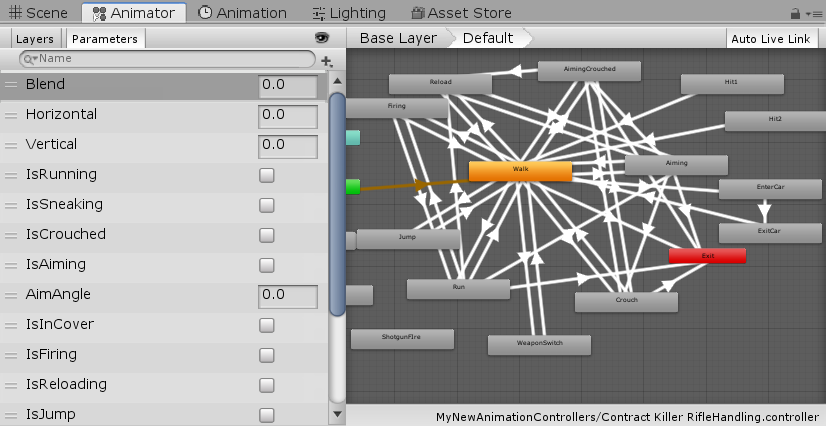
\includegraphics[width=0.6\linewidth,clip=]{slike/AnimatorController.png}
\figcaption{Kontroler animacija}%
\label{fig:AnimatorController}%
\end{minipage}
\\[\intextsep]
Jedan od standardnih zadataka kada su u pitanju animacije je miješanje jedne ili više sličnih animacija, za to nam služi stablo miješanja animacija (engl.~\textit{Blend tree}). Možda najpoznatiji primjer je miješanje između hodanja i trčanja ovisno o brzini lika, drugi primjer je naginjanje lika lijevo ili desno dok trči itd. Važno je razlikovati tranzicije između stanja i stabla miješanja, iako i jedno i drugo služi za glatki prijelaz između animacija, koriste se u različitim situacijama. Dok tranzicije služe za prijelaz između stanja unutar nekog perioda vremena, miješanje se događa korištenjem više animacija te ovisno o vrijednosti određenih parametara dobiva se konačni izgled animacije. 
Može se odabrati 1D ili 2D miješanje, ovisno o odabranom, bit će potrebno mijenjati vrijednost, jednog ili više parametara. Osim toga rad sa stablom je sličan radu sa stanjima, a to je dodavanje stanja unutar stabla, te dodavanjem animacije. Na slikama ~\ref{fig:BlendTree} i ~\ref{fig:AnimatorBlend} prikazan je prozor stabla miješanja animacija.
\\[\intextsep]
\begin{minipage}{\linewidth}
\centering%
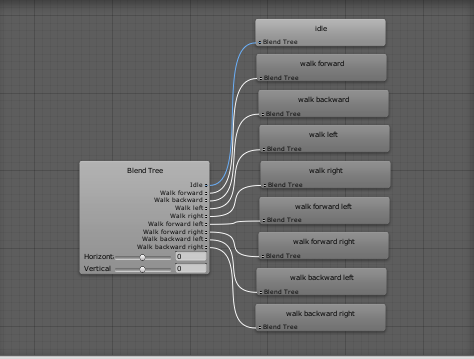
\includegraphics[width=0.6\linewidth,clip=]{slike/BlendTree.png}
\figcaption{Nazivi animacija}%
\label{fig:BlendTree}%
\end{minipage}
\\[\intextsep]
\\[\intextsep]
\begin{minipage}{\linewidth}
\centering%
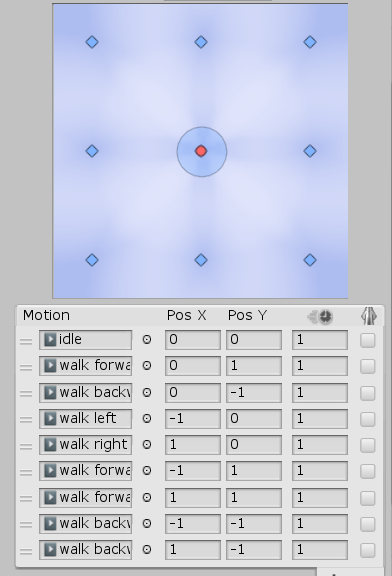
\includegraphics[width=0.6\linewidth,clip=]{slike/BlendTreeParam.png}
\figcaption{Animacije i parametri}%
\label{fig:AnimatorBlend}%
\end{minipage}
\\[\intextsep]

Ovisno o tome koliko je kompleksan izrađeni sustav animacija, moguće je stvoriti više slojeva animacija, te onda razdvojiti slojeve ovisno o tome u kojem je stanju lik, dakle moguće je napraviti npr. sloj nenaoružan lik, dodati odgovarajuća stanja, te ako je lik naoružan, sloj gdje će biti stanja sukladno tome.

Sistem navigacije u Unityju omogućava stvaranje prohodnog područja na osnovu geometrije unutar scene. Tako je moguće dodavati likove koji će se korištenjem sistema pronalaženja puta kretati unutar scene prema određenim pravilima, što uključuje zaobilaženje prepreka, zaustavljanje na rubovima, skakanje i slično.

Ovaj sustav se sastoji od idućih komponenti:
\begin{itemize}
  \item NavMesh je struktura podataka koja opisuje površine gdje se može kretati, te omogućava pronalaženje puta iz jednog područja gdje je dopušteno kretati se u drugo. Ovaj podatak se automatski generira na osnovi geometrije levela.
  \item NavMesh Agent je komponenta koja pomaže pri stvaranju likova koji mogu izbjegavati jedan drugog tijekom kretanja prema cilju, kao i izbjegavanje bilo kojih drugih prepreka
  \item Off-Mesh Link je komponenta koja omogućava korištenje prečaca tijekom kretanja,a koji ne mogu biti prikazani kao površina gdje je omogućeno kretanje, kao što je skakanje preko ograde, ili otvaranje vrata itd.
  \item NavMesh Obstacle je komponenta kojom je moguće opisati prepreke koje bi lik trebao izbjegavati tijekom kretanja kroz svijet, a da se kreču prema liku, ili ako je riječ o statičnom objektu onda omogućava jednostavno pronalaženje drugog puta
\end{itemize}

Korištenje ovog sustava u projektu se radi tako da se doda prozor za navigaciju, potom se ispeče (engl.~\textit{Bake}), dakle napravi se mapa (NavMesh) bazirana na geometriji levela, potom se objektu za kojeg želite da se kreče po ovoj mapi doda komponenta NavMesh Agent te se konfiguriraju postavke vidljive na slici ~\ref{fig:NavMeshAgentSetup}.
\\[\intextsep]
\begin{minipage}{\linewidth}
\centering%
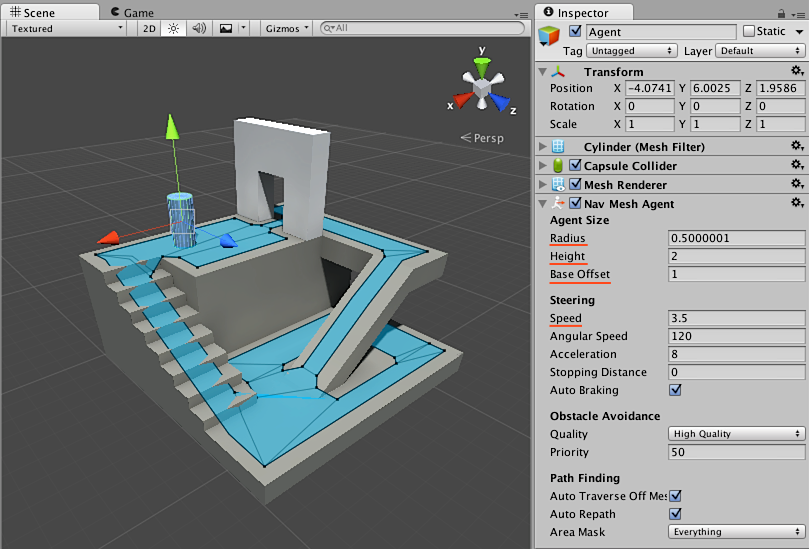
\includegraphics[width=0.6\linewidth,clip=]{slike/NavMeshSetUp.png}
\figcaption{NavMesh mapa i agent}%
\label{fig:NavMeshAgentSetup}%
\end{minipage}
\\[\intextsep]

Plavom bojom je obojeno područje gdje se agent može kretati,a u postavkama se konfigurira sami agent, veličina, inteligencija, pronalaženje puta i brzina. Sve što je potrebno sada da se agent kreče je napisati logiku unutar skripte, ispod je jednostavan primjer kako možemo koristiti komponentu NavMesh Agent. ~\ref{MoveTo}.
\begin{lstlisting}[caption={Korištenje navigacije}, label=MoveTo];
using System.Collections;
    
public class MoveTo : MonoBehaviour {
       
public Transform goal;
       
	void Start () {
	NavMeshAgent agent = GetComponent();
	agent.destination = goal.position; 
       }
}
\end{lstlisting}
Za napraviti NavMesh Obstacle, odnosno prepreku, treba dodati istoimenu komponentu objektu kojeg je potrebno izbjeći, potom je potrebno podesiti određene postavke, odabrati oblik te dodati Rigidbody komponentu i na kraju postaviti Carve kako bi agent mogao pronaći put pored prepreke. Jednako se postupa prilikom stvaranja Off Mesh Linka, doda se pozicija gdje je omogućeno preskakanje ograde ili skakanje s visine, postavi se pozicija gdje završava ta radnja, objektu koji se nalazi na startnoj poziciji doda se istoimena komponenta te postave potrebne vrijednosti, odnosno startna i krajnja pozicija i to je to. Agent će tijekom kretanja iskoristiti tu mogućnost ako je to brži put prema cilju.
Kako bi se dobila što precizniju mapu kretanja potrebno je omogućiti računanje visinske mape unutar postavki za pečenje. Isto tako je moguće postaviti različite vrijednosti određenih pozicija mape, tako da ako agent naiđe na površine s većom vrijednosti pokušat će pronaći neki drugi put. Unity koristi A* algoritam za računanje najkraćeg puta do cilja, a radi tako da koristi graf povezanih čvorova, algoritam započinje s najbližim čvorom početku puta te posjećuje povezane čvorove sve dok ne dođe do cilja. Vrijednost, odnosno cijena kretanja između dva čvora ovisi o udaljenosti te cijeni vezanu za područje gdje se agent kreče, ako je cijena npr. 2.0, tada će se ukupna vrijednost računati kao dvostruko duža od 1.0, tako da je moguće postaviti različite cijene na mapi ako želimo specificirati put kojim će se agent kretati.

Unity omogućava vrlo jednostavnu izradu korisničkog sučelja u igri, bilo to vezano za različite izbornike ili prikaz osnovnih informacija tijekom igranja. 
Glavna komponenta korisničkog sučelja (UI) je platno (engl.~\textit{Canvas}), to je prostor gdje bi se trebali nalaziti svi elementi grafičkog sučelja. To je objekt igre koji sadrži komponentu Canvas, a svi ostali elementi su djeca platna. Platno se unutar scene prikazuje kao pravokutnik te je najjednostavnije raditi s platnom tako da se postavi 2D prikaz unutar scene. Elementi se crtaju na platnu redoslijedom kako se pojavljuju u hijerarhiji, što znači da ako se dva elementa preklapaju, onaj kasnije naveden bit će nacrtan preko prijašnjeg. Tri su načina učitavanja platna, a to su prevlačenje, dakle ako je promijenjena rezolucija, promijenit će se i veličina platna. Kamera, učitava se ovisno o tome koliko je platno udaljeno od određene kamere i o postavkama kamere. A treći način je prostor svijeta, odnosno platno se ponaša kao bilo koji drugi objekt unutar scene, moguće je ručno mijenjati veličinu svih elemenata, te će se učitavati ovisno o tome jesu li ispred ili iza nekog objekta u sceni.
Pozicija elementa je definirana preko sidrišta (engl.~\textit{Anchor}), dakle element se usidri na određenoj poziciji, npr. gore desno, te neovisno o veličini ekrana, i rezoluciji, taj element će uvijek gravitirati toj poziciji. Tako smo sigurni da bez obzira na postavke igranja, element će uvijek biti prisutan na očekivanoj poziciji. Kao i kod ostalih objekata, promjene nad roditeljem, utječu i na djecu.
Neke od standardnih komponenti platna su:
\begin{itemize}
  \item Tekst, kao što i samo ime sugerira, element koji sadrži određeni tekst.
  \item Slika, nije obična tekstura već (engl.~\textit{Sprite}), može služiti kao pomična slika za prikaz stanja lika i slično.
  \item Standardna slika (engl.~\textit{RawImage}), prima jednostavno teksturu za prikaz.
  \item Botuni, koriste se za standardne radnje kao što su pokretanje različitih događaja, mijenjanje postavki itd.
  \item Klizači, kao i botuni, mogu se koristiti za promjene postavki, a u kombinaciji sa slikama služe za izradu stanja energije (engl.~\textit{Health bar}).
\end{itemize}
Svim navedenim elementima moguće je upravljati preko skripti, te ih animirati, bilo to zacrnjivanje slike preko cijelog ekrana tijekom mijenjanja scene, ili prikaz različitih pomičnih elemenata unutar izbornika, kao i za prikaz svih dinamičkih podataka u stvarnom vremenu igraču. Na slici~\ref{fig:Canvas} prikazano je grafičko sučelje Dionyzus igre sa svim najvažnijim podacima potrebnim tijekom igranja.
\\[\intextsep]
\begin{minipage}{\linewidth}
\centering%
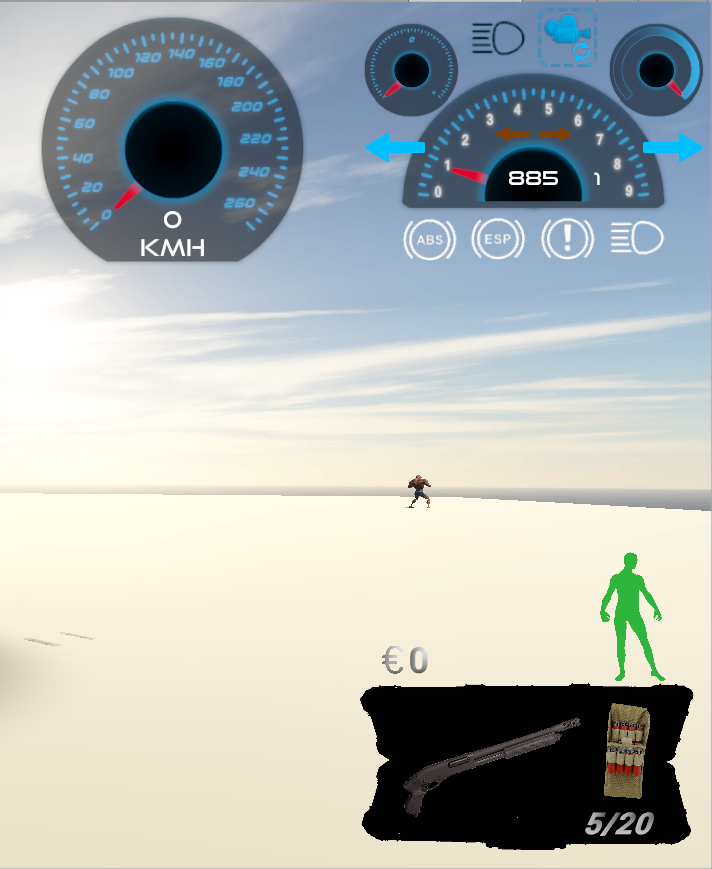
\includegraphics[width=0.6\linewidth,clip=]{slike/Canvas.png}
\figcaption{Grafičko sučelje}%
\label{fig:Canvas}%
\end{minipage}
\\[\intextsep]
Skripte su nužan dio svih igara. Čak i u najjednostavnijim igrama je potrebno napisati skripte koje će opisivati kako će igra reagirati prilikom unosa korisnika, kako i zašto će se dogoditi određeni događaji itd. Osim toga skripte se mogu koristiti za stvaranje grafičkih efekata, za kontroliranje ponašanje objekata kao i za implementiranje inteligencije likova u igri.
U ovom poglavlju će biti opisani glavni koncepti vezani za pisanje skripti u te s tim završava opisivanje rada unutar Unityja.
Ponašanje objekata igre je kontrolirano od strane komponenti koje sadrži taj objekt, iako je s ugrađenim komponentama moguće stvoriti raznovrsne elemente igre, vrlo brzo dolazi do potrebe stvaranja vlastite logike.
Skritpe se stvaraju tako da se unutar dodataka doda nova C\# skripta te joj se dodjeli ime. Nakon stvaranja skripte automatski se generira kostur unutar skripte prikazan u dijelu k\^oda ispod~\ref{MonoBehaviour}.
\begin{lstlisting}[caption={Nova skripta}, label=MonoBehaviour];
using UnityEngine;
using System.Collections;

public class MainPlayer : MonoBehaviour {

    // Use this for initialization
    void Start () {
    
    }
    
    // Update is called once per frame
    void Update () {
    
    }
}
\end{lstlisting}
Dakle svaka novo stvorena skripta sadrži istoimenu klasu koja implementira klasu MonoBehaviour. MonoBehaviour je nacrt za stvaranje nove komponente koja se može dodavati na bilo koji objekt igre. Važno je da su naziv klase i datoteke jednaki kako bi se omogućila funkcionalnost te skripte.
Isto tako generirane su dvije metode bez tijela. Unutar Update se piše k\^od koji je će upravljati ažuriranjem objekta igre kroz vrijeme. To može biti kretanje, okidanje različitih akcija ili reagiranje na korisnikov unos. Start metoda se poziva prije početka igre, odnosno prije prvog poziva Update metode te je idealna za bilo kakvu vrstu inicijalizacije. Nije potrebno pisati konstruktore jer se o tome brine Unity editor, a pisanjem vlastitih konstruktora može uzrokovati poremećaj normalne funkcionalnosti Unityja. Kako bi aktivirali logiku napisanu unutar skripte potrebno ju je dodati na objekt gdje želimo da se primjeni napisana logika.
Kao i sve ostale komponente skripte mogu imati svojstva koja je moguće mijenjati unutar nadglednog prozora, što je prikazano na slici~\ref{fig:EditingVarInspector}.
\\[\intextsep]
\begin{minipage}{\linewidth}
\centering%
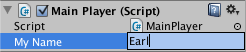
\includegraphics[width=0.6\linewidth,clip=]{slike/EditingVarInspector.png}
\figcaption{Prikaz skripte s javnom varijablom}%
\label{fig:EditingVarInspector}%
\end{minipage}
\\[\intextsep]
K\^od ispod~\ref{Varijabla} sadrži logiku skripte iznad, dakle dodana je javna varijabla myName te je unutar startne metode jednostavno ispisana koristeći Debug.Log metodu.
\begin{lstlisting}[caption={Dodavanje javne varijable}, label=Varijabla];
using UnityEngine;
using System.Collections;

public class MainPlayer : MonoBehaviour 
{
    public string myName;
    
    // Use this for initialization
    void Start () 
    {
        Debug.Log("I am alive and my name is " + myName);
    }
}
\end{lstlisting}
Unity dopušta mijenjanje vrijednosti tijekom igranja, što je jako korisno za testiranje različitih efekata, ili prilagođavanje određenih pozicija i slično. Ono što je moguće preko skripte, a ne i u editoru je mijenjanje vrijednosti tijekom vremena. Najčešći i najjednostavniji način pristupanja komponentama unutar k\^oda je prikazan je ispod~\ref{GetComponent}.
\begin{lstlisting}[caption={Dodavanje javne varijable}, label=GetComponent];
void Start ()
{
    Rigidbody rb = GetComponent();
    
    // Add a force to the Rigidbody.
    rb.AddForce(Vector3.up * 10f);
}
\end{lstlisting}
Na ovaj način se može dohvatiti bilo koja komponenta koju sadrži objekt, isto tako je moguće imati više od jedne skripte na jednom objektu. Ako je potrebno koristiti neki objekt igre unutar skripte, potrebno je deklarirati objekt tipa GameObject, te mu onda pridružiti odgovarajuću vrijednost, to može biti javna varijabla kojoj će se dodijeliti odgovarajući objekt u samom editoru, ili dohvačanje objekta preko imena ili taga.
Ono što je karakteristično za skripte je što Unity daje kontrolu skripti tako što poziva funkcije koje su deklarirane u samoj skripti, a u trenutku kada funkcija završava, kontrola se predaje nazad Unityju. Te funkcije su tzv. funkcije događaja, pošto se aktiviraju kao odgovor prilikom određenog događaja tijekom igranja. Neke od tih funkcija su Start i Update funkcije. Update se poziva prije učitavanja trenutka i prije računanja animacije, isto tako postoji FixedUpdate koji se poziva prije ažuriranje fizike. Pošto se fizika i trenutka ne ažuriraju s istom frekvencijom, precizniji se rezultati dobivaju ako se k\^od vezan za fiziku napiše unutar FixedUpdate metode. Kada je potrebno napraviti dodatne promjene nakon Update ili FixedUpdate funkcija, npr. kada je kameru potrebno prilagoditi nakon što se ciljani objekt pomaknuo, ali ne u isto vrijeme, ili ako je u k\^odu potrebno pregaziti efekt animacije, npr. postaviti glavu lika da gleda prema nekom objektu u sceni. U tim slučajevima je najbolje koristiti LateUpdate metodu. Osim navedenih postoji i Awake metoda koja se poziva u trenutku učitavanja scene, što znači da će sve Awake metode biti pozvane prije prve Start metode. Tada je moguće unutar Start metode napraviti logiku koja će koristiti neku od inicijalizacija napravljenih u Awake.

Osim standardnih metoda za upravljanje događajima postoje i one za upravljanje grafičkim sučeljem. Neke od metoda su OnGUI, a one što su korištene i u samom projektu su OnMouseOver i OnMouseDown, ovim metodama možemo kontrolirati što će se dogoditi kada je pokazivač miša usmjeren prema određenom objektu, npr. za okidanje događaja koji će prikazati tekstualni sadržaj ili omogućiti pritisak nekog botuna kako bi se pokrenuo neki događaj.

Kada je riječ o pokretanju objekata i upravljanju vremena, važno je voditi računa o tome da frekvencija učitavanja nije uvijek ista. Dakle nije moguće postaviti fiksne vrijednosti koliko će puta preči neki lik u određenom periodu vremena, već je potrebno uzeti u obzir i frekvenciju, za to se koristi svojstvo \texttt{ Time.deltaTime }.
U kratkom primjeru ispod~\ref{Time} prikazano je kako se koristi ovo svojstvo, odnosno koji je ispravan pristup kada je riječ o upravljanju objekata tijekom vremena u igri.
\begin{lstlisting}[caption={Upravljanje vremenom}, label=Time];
using UnityEngine;
using System.Collections;

public class ExampleScript : MonoBehaviour {
    public float distancePerSecond;
    
    void Update() {
        transform.Translate(0, 0, distancePerSecond * Time.deltaTime);
    }
}
\end{lstlisting}
Moguće je mijenjati fiksni pomak vremena, \texttt{ Time.fixedDeltaTime }. Ako je zadan veliki posao za stroj fizike, onda je moguće smanjiti početnu vrijednost, ali to zahtjeva veći rad procesora. Isto tako je moguće povećati vrijednost, tijela koja su pod utjecajem fizike neće savršeno reagirati na promjene, ali to nije toliko primjetno te je prihvatljivo s obzirom na to da to može poboljšati performans igre.

Postoji još jedan način upravljanja vremenom a to je korištenje \texttt{ Time.timeScale }svojstva, tim svojstvom mijenjamo koliko brzo ide vrijeme unutar igre s obzirom na stvarno vrijeme. Ovime je moguće ubrzati ili usporiti kretnje objekata u igri, npr. moguće je napraviti sporije animacije (engl.~\textit{Slow motion}), ubrzati neke radnje tijekom kratkih filmova te isto tako kompletno pauzirati igru.
Navedene opcije mogu se mijenjati i globalno unutar prozora Time, odnosno vrijeme, ali je puno bolji pristup upravljanje ovim svojstvima unutar skripti. Primjer k\^oda~\ref{timeScale}
\begin{lstlisting}[caption={Upravljanje vremenom}, label=timeScale];
using UnityEngine;
using System.Collections;

public class ExampleScript : MonoBehaviour {
    void Pause() {
        Time.timeScale = 0;
    }
    
    void Resume() {
        Time.timeScale = 1;
    }
}
\end{lstlisting}
Upravljanje objektima često je vezano za njihovo pojavljivanje i brisanje iz scene, za to je moguće koristiti metode kao što su Instantiate za stvaranje objekta u određenim situacijama, npr. metak, kontrast tome je metoda Destroy, koja kao što joj i naziv govori uništava objekt, odnosno briše ga kompletno iz scene, tako je moguće riješiti se nepotrebnih objekata, te optimizirati igru. Ako je potrebno samo trenutno onesposobiti neki objekt, ili aktivirati samo u određenim situacijama, tada je moguće koristiti metodu setActive koja prima boolean true ili false.

Za određene efekte, kao što su zacrnjivanje ekrana, ili jednostavno tok teksta koji se prikazuje na ekranu, standardne metode nisu dovoljno dobre, svaka metoda se odradi unutar jednog trenutka vremena te je nemoguće prikazati promjene trenutak po trenutak. U tom slučaju potrebno je koristiti metode koje mogu odraditi dio skripte, potom dati kontrolu Unity, te nakon određenom perioda opet odraditi nastavak skripte, to su (engl.~\textit{Coroutine}), a nalaze se u IEnumerator sučelju. Primjer korištenja je u skripti ispod~\ref{Coroutine}.
\begin{lstlisting}[caption={Upravljanje vremenom}, label=Coroutine];

    public int waitTimeForCredits = 3;
    public float waitTimeForCameraSwitch = 5f;
    public float waitForThirdCamera = 3f;

	// Use this for initialization
	void Start () {
        StartCoroutine(CameraSwitcher());
	}

    IEnumerator CameraSwitcher()
    {
        yield return new WaitForSeconds(waitTimeForCredits);
        credLeadDesigner.SetActive(true);

        yield return new WaitForSeconds(waitTimeForCredits);
        credStory.SetActive(true);

        yield return new WaitForSeconds(waitForThirdCamera);
        thirdCamera.SetActive(true);
        firstCamera.SetActive(false);

        yield return new WaitForSeconds(2);
        credEngine.SetActive(true);


        yield return new WaitForSeconds(waitTimeForCameraSwitch);
        secondCamera.SetActive(true);
        thirdCamera.SetActive(false);
        credGameName.SetActive(true);

        yield return new WaitForSeconds(6);
        secondCamera.SetActive(false);
        fourthCamera.SetActive(true);

        yield return new WaitForSeconds(9.5f);
        fourthCamera.SetActive(false);
        fifthCamera.SetActive(true);
    }
\end{lstlisting}

Dakle korištenjem metode WaitForSeconds odgađamo vrijeme te dajemo kontrolu Unityju, a nakon što završi taj period vremena, opet se izvršava k\^od u skripti, kao što je vidljivo u skripti ovo je korisno ako želite uključiti ili isključiti određene objekte u sceni, te za stvaranje različitih efekata. Osim toga korištenjem IEnumeratora moguće je različite zahtjevne zadatke rasporediti te tako poboljšati performanse igre.

Vektorska aritmetika je osnova za 3D grafiku, fiziku i animaciju, Unity ima implementirane sve najvažnije funkcionalnosti za rad s vektorima, a to su zbrajanje, oduzimanje, množenje i normalizacija vektora i slično. Pa se tako oduzimanje vektora može koristiti kada je potrebno izračunati udaljenost između dva objekta, a za određivanje smjera se koristi normalizacija vektora. Još jedan od primjera korištenja vektora je prilikom mjerenja brzine automobila, to se uglavnom radi tako da se mjeri brzina rotiranja kola, međutim ako automobil ne ide pravo, odnosno klizi sa strane tada ne možemo dobiti točan rezultat brzine. Međutim korištenjem metode, odnosno računanjem skalarnog produkta vektora, ova metoda ne koristi sporu metodu korjenovanja, što znači da nije zahtjevna za konstantno ažuriranje.
Za traženje grešaka moguće je postaviti nadgledni prozor u Debug način rada, a isto tako Visual Studio ima ugrađeni program za pronalaženje grešaka (engl.~\textit{Debugger}). Osim toga Unity ima svoj konzolni prozor gdje se ispisuju pogreške kao i upozorenja, te je isto tako moguće ispisivati poruke unutar konzole koristeći \texttt{ Debug.Log } funkcionalnost.
Više o samom pisanju skripti bit će opisano u dijelu opisivanja samog projekta, gdje će se prikazati pristup prilikom rješavanja konkretnih problema tijekom izrade igre.

Ovim završava opisivanje općenitog rada u Unityju te će u nastavku biti opisan sami projekt.